\subsection{Exploring the Curious Case of Coaxial Cable Lengths!}

\begin{tcolorbox}[colback=gray!10, colframe=black, title=E9F03] 

Why is the electrical length of a coaxial cable longer than its physical length?  
\begin{enumerate}[label=\Alph*.]
    \item Skin effect is less pronounced in the coaxial cable
    \item Skin effect is more pronounced in the coaxial cable
    \item Electromagnetic waves move faster in coaxial cable than in air
    \item \textbf{Electromagnetic waves move more slowly in a coaxial cable than in air}
\end{enumerate} \end{tcolorbox}

\subsubsection*{Related Concepts}

To understand why the electrical length of a coaxial cable is longer than its physical length, we first need to discuss a few key concepts in electromagnetic theory and wave propagation.

1. \textbf{Electrical Length vs. Physical Length:}: 
   The electrical length of a transmission line (such as coaxial cable) describes how long the line appears to an electromagnetic wave. It takes into account the velocity of the signal as it travels through the medium.

2. \textbf{Speed of Electromagnetic Waves:}: 
   The speed of a wave in a transmission medium is determined by the properties of the material through which it propagates. In air, electromagnetic waves travel at approximately the speed of light \( c \approx 3 \times 10^8 \, \text{m/s} \). However, when these waves propagate through any dielectric material, like the insulating material in coaxial cables, their speed decreases due to the medium's permittivity and permeability.

3. \textbf{Dielectric Constant:}: 
   The dielectric constant (\( \epsilon_r \)) of a material is a measure of its capacitance compared to a vacuum. The speed of light in a medium can be calculated using:
   \[
   v = \frac{c}{\sqrt{\epsilon_r}}
   \]
   where \( v \) is the speed of the electromagnetic wave in the medium.

4. \textbf{Coaxial Cable Properties:}: 
   A coaxial cable generally has a dielectric material that slows down the electromagnetic waves more than air does. Thus, the effective velocity of signal propagation in a coaxial cable is less than that in free space.

Given these points, the correct answer to the question is choice D: Electromagnetic waves move more slowly in a coaxial cable than in air.

\subsubsection*{Calculation of Electrical Length}

If we consider a coaxial cable with a certain dielectric constant, we can illustrate the relationship between physical length, electrical length, and signal speed. For example, if the physical length of a coaxial cable is \( L \) and the dielectric constant is \( \epsilon_r = 2.25 \) (which is a typical value for some insulating materials):

The speed of light in the coaxial cable can be calculated as follows:
\[
v = \frac{c}{\sqrt{\epsilon_r}} = \frac{3 \times 10^8}{\sqrt{2.25}} \approx 2 \times 10^8 \, \text{m/s}
\]

Now, if we want to find the electrical length \( L_{el} \) corresponding to a physical length \( L = 1 \, \text{m} \):
\[
L_{el} = \frac{L}{\sqrt{\epsilon_r}} = \frac{1}{\sqrt{2.25}} \approx 0.6667 \, \text{m}
\]
This means that the electrical length appears longer due to the slower transmission of electromagnetic waves within the coaxial cable.

\subsubsection*{Diagram}

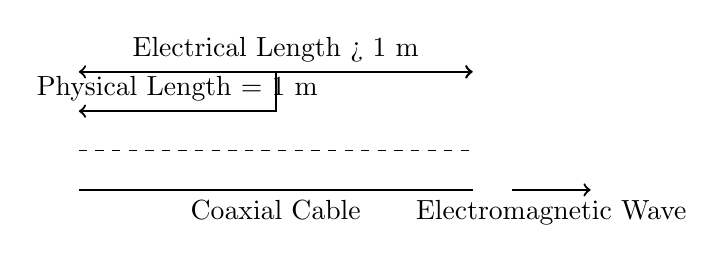
\begin{tikzpicture}
    \draw[thick] (0,0) -- (5,0) node[midway, below] {Coaxial Cable};
    \draw[dashed] (0,0.5) -- (5,0.5);
    \draw[->, thick] (5.5,0) -- (6.5,0) node[midway, below] {Electromagnetic Wave};
    \draw[<->, thick] (0,1) -- (2.5,1) node[midway, above] {Physical Length = 1 m} -- (2.5,1.5) -- (5,1.5) ;
    \draw[<->, thick] (0,1.5) -- (5,1.5) node[midway, above] {Electrical Length > 1 m};
\end{tikzpicture}
